\chapter{Implementación}

\section{Estructura de nuestro frontend}
Se ha utilizado github y git para tener nuestra propia versión de JPLAG en nuestra cuenta de Github (https://github.com/AntonioJavierRP), gracias a esto podremos realizar los cambios que veamos necesarios en nuestra versión y mandar un pull request al repositorio original en \cite{jplag_github} por si el autor quiere incorporar el frontend que hemos creado para R a su versión.
\newline
Los cambios y las pruebas hechas en dicho código se han realizado en nuestra propia máquina local.
\newline
Nuestro frontend consta de la estructura de archivos que podemos ver en la Figura \ref{fig:ej_frontend} basada en los frontends ya existentes, especialmente en el de Java 1.7 y Python 3, ya que usan la misma herramienta que nosotros para crear el analizador sintáctico.

\begin{figure}[H] %con el [H] le obligamos a situar aquí la figura
\centering
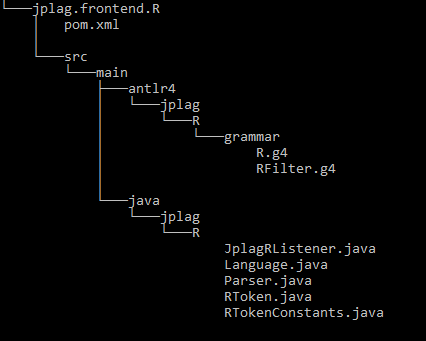
\includegraphics[scale=1]{imagenes/estructura_frontend.png}  %el parámetro scale permite agrandar o achicar la imagen. En el nombre de archivo puede especificar directorios
\caption{Árbol de archivos del frontend creado} \label{fig:ej_frontend}
\end{figure}

Como se puede apreciar, nuestro frontend consta de 8 archivos:
\begin{itemize}
\item \textbf{pom.xml}: archivo con la opciones de construcción y compilación de nuestro frontend en JPLAG.
\item \textbf{R.g4}: archivo de gramática que representa a R procesado por ANTLR4.
\item \textbf{RFilter.g4}: otro archivo de gramática que representa a R procesado por ANTLR4.
\item \textbf{JplagListener.java}: este archivo se encarga de seleccionar los tokens que mejor representan al lenguaje.
\item \textbf{Languaje.java}: en este archivo constan las características del lenguaje que JPLAG debe de saber antes de procesar los archivos enviados.
\item \textbf{Parser.java}: este archivo se encarga de extraer los tokens y de enviárselos a JPLAG.
\item \textbf{RToken.java y RTokenConstants.java}: en estos archivo especificamos los tokens importantes de R.
\end{itemize}
En los siguientes apartados se explica en más profundidad la función de cada uno de estos archivos.


\subsection{Apache Maven}

Para la construcción y gestión de JPLAG el autor original ha usado Maven.
\newline
Apache Maven es una herramienta de gestión y comprensión de proyectos software en Java \cite{maven_web}, es decir, es lo que se encarga de que se compilen todos los fuentes correctamente.
\newline
Maven permite la construcción de proyectos a través de archivos POM (project object model) y de un conjunto de plugins que tienen todos los proyectos que usan Maven (tiene que ser instalado previamente).
\newline
Un archivo pom.xml tiene una estructura básica similar a la que se muestra en el ejemplo a continuación en la Figura \ref{fig:ej_POM}.

\begin{figure}[H] %con el [H] le obligamos a situar aquí la figura
\centering
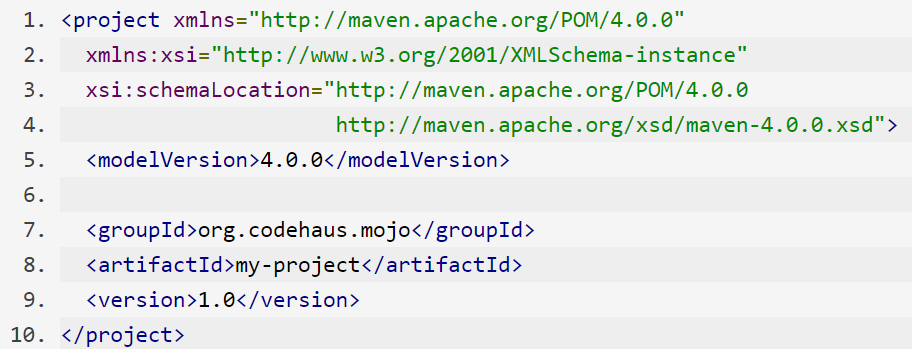
\includegraphics[scale=0.55]{imagenes/estructura_POM.png}  %el parámetro scale permite agrandar o achicar la imagen. En el nombre de archivo puede especificar directorios
\caption{Archivo ejemplo pom.xml} \label{fig:ej_POM}
\end{figure}

Para que nuestro frontend se tuviese en cuenta cuando se construye el proyecto se han tenido que modificar tres de los archivos pom.xml ya existentes en el proyecto añadiéndoles dependencias y módulos.
\newline
Así mismo se ha tenido también que crear nuestro propio archivo pom.xml dentro de nuestra carpeta del frontend como ya vimos en la Figura \ref{fig:ej_frontend}.

\section{Analizador utilizado}

Como ya mencionamos anteriormente, el frontend se encarga de reconocer las cadenas de tokens para que se les pueda aplicar el algoritmo. Para poder identificar estos tokens necesitamos un parser (analizador sintáctico).
\newline
En el resto de frontends los parser creados se han hecho usando JAVACC o ANTLR.
\newline
Estas son herramientas para la creación de analizadores de lenguajes basándose en gramáticas.
Para la creación de nuestro analizador sintáctico de R hemos escogido ANTLR4.



\subsection{ANTLR}
ANTLR (ANother Tool for Language Recognition) es un generador de analizadores sintácticos desarrollado por Terrence Parr \cite{antlr_libro}. 
\newline
Un analizador sintáctico procesa un trozo de texto y lo transforma en una estructura organizada, en un árbol de sintaxis. Este árbol representa la estructura lógica del contenido del código que ha procesado. Un ejemplo de tal árbol es el que vemos en la Figura \ref{fig:arbol_euclides} en el que se representa el código del algoritmo de Euclides.


\begin{figure}[] %con el [H] le obligamos a situar aquí la figura
\centering
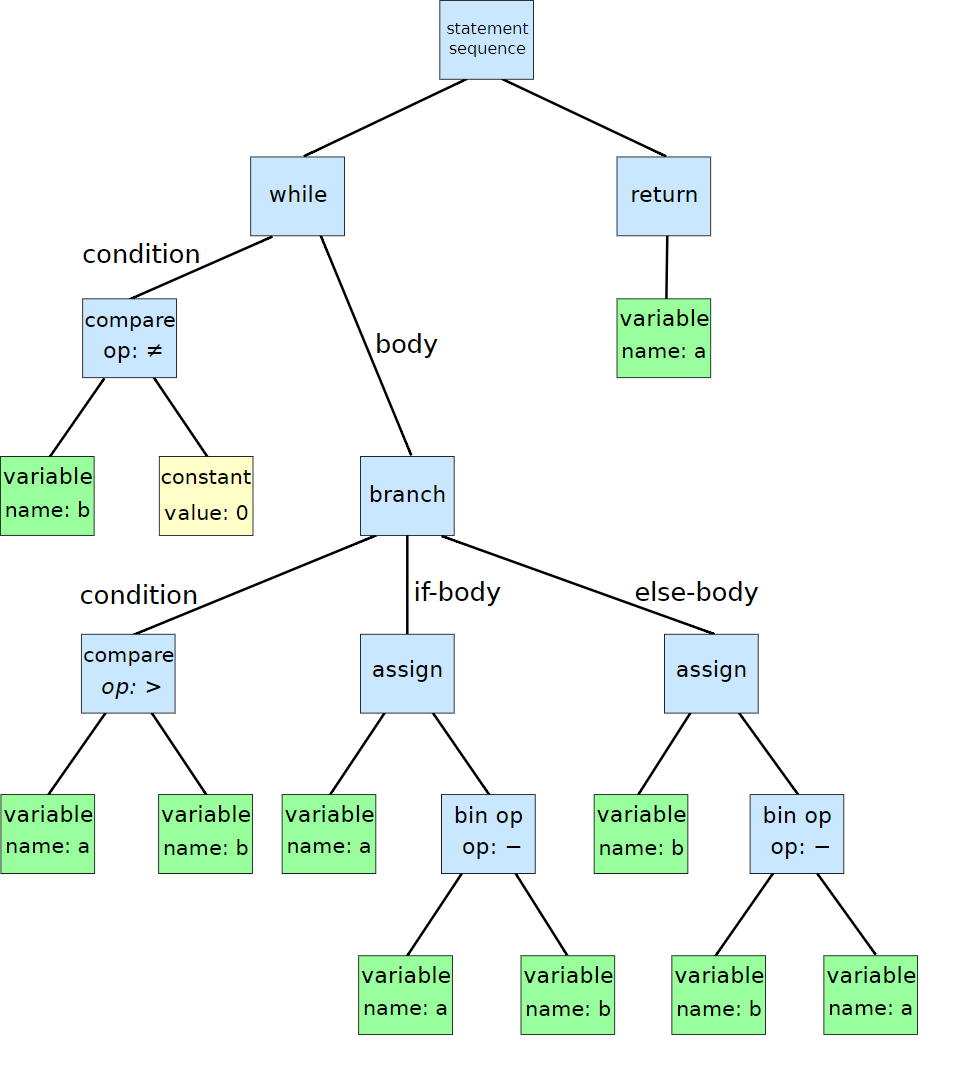
\includegraphics[scale=0.55]{imagenes/arbol.png}  %el parámetro scale permite agrandar o achicar la imagen. En el nombre de archivo puede especificar directorios
\caption{Árbol de sintaxis del algoritmo de Euclides.} \label{fig:arbol_euclides}
\end{figure}


Para obtener un árbol de sintaxis necesitaremos definir una gramática, invocar a ANTLR, para que genere un parser a partir de esta, y pasarle el código del que quieres obtener el árbol al parser.
\newline

ANTLR4 es la versión 4 de ANTLR y aporta numerosas nuevas funcionalidades que reducen la curva de aprendizaje necesaria para desarrollar la gramática de tu lenguaje. 
\newline
La característica más importante de esta versión es que acepta cualquier gramática que le hagas procesar a excepción de gramáticas con recursión indirecta por la izquierda (esto se da cuando una regla referencia a otra regla a la izquierda y esta segunda regla termina referenciando a la primera sin llegar a un símbolo terminal o token).
\newline
Los archivos que contienen la gramática tendrán que tener la extensión .g4, el nombre de la gramática como nombre del archivo y empezar con la línea de código : grammar $<nombre del archivo>$; . Aunque también puede comenzar siendo un parser grammar o lexer grammar si sólo vamos a definir reglas del analizador léxico o sintáctico. En nuestro caso el archivo se llama R.g4 y el archivo empieza con grammar R;.
\newline
El resto del archivo contendrá reglas del analizador léxico (lexer rules) y reglas del analizador sintáctico (parser rules).

\bigskip

Las ''lexer rules'' son las definiciones de los tokens básicos que conforman el lenguaje y siguen la sintaxis de las reglas sintácticas. Las reglas del analizador léxico se escriben en mayúscula y al final del archivo, en Figura \ref{fig:lexer_rules} podemos ver un ejemplo de estas reglas.

\begin{figure}[] %con el [H] le obligamos a situar aquí la figura
\centering
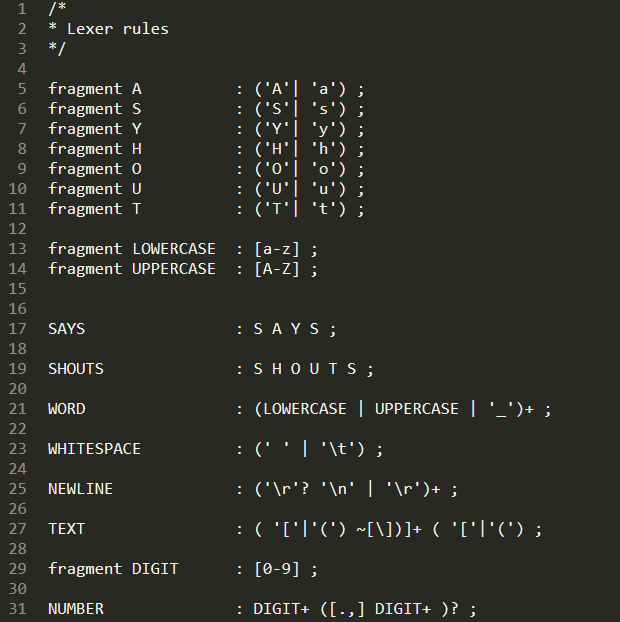
\includegraphics[scale=0.55]{imagenes/lexer_rules.png}  %el parámetro scale permite agrandar o achicar la imagen. En el nombre de archivo puede especificar directorios
\caption{Ejemplo de lexer rules.} \label{fig:lexer_rules}
\end{figure}

\bigskip

Las ''parser rules'' son la reglas que muestran las combinaciones posibles de los tokens básicos (definidos en las lexer rules) en el lenguaje.
\newline
Tenemos una primera regla (en el ejemplo que mostramos es 'chat') que genera el resto de reglas.
Estas reglas se escriben en minúsculas y se deben de poner antes que las reglas del analizador léxico.
\newline
Podemos ver un ejemplo de estas en la Figura \ref{fig:parser_rules}.

\begin{figure}[] %con el [H] le obligamos a situar aquí la figura
\centering
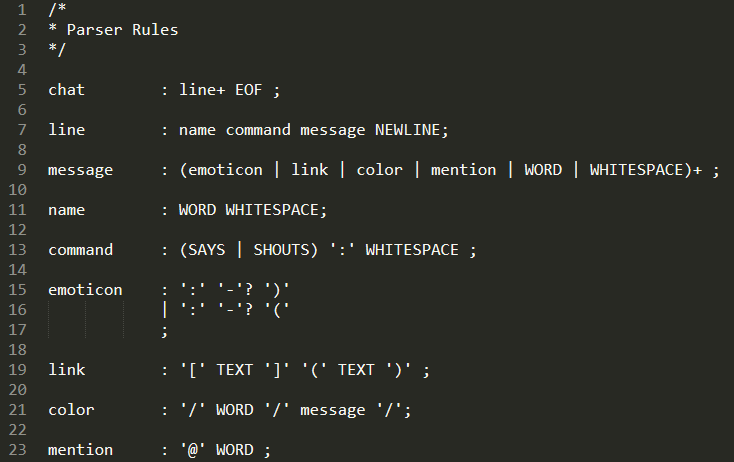
\includegraphics[scale=0.55]{imagenes/parser_rules.png}  %el parámetro scale permite agrandar o achicar la imagen. En el nombre de archivo puede especificar directorios
\caption{Ejemplo de parser rules.} \label{fig:parser_rules}
\end{figure}


\section{Adaptación del parser a JPLAG}

La gramática que hemos usado se encuentra en el archivo R.g4 junto con RFilter.g4.
Nuestra gramática está basada en una ya existente para R en ANTLR4 encontrada en \cite{repositorio_gramatica}. Hemos añadido una gran cantidad de reglas del análisis sintáctico nuevas en el archivo R.g4 para poder quedarnos con los tokens más representativos del lenguaje ya que necesitamos que los tokens que estamos agrupando aparezcan agrupados como parser rule, como por ejemplo, en el caso de los tokens para el flujo de control ''if''. Hemos creado la siguiente regla:

\begin{center}
\begin{lstlisting}
if_statement :  'if' '(' expr ')' expr | 'if' '(' expr ')' expr 'else' expr ;
\end{lstlisting}
\end{center}

Esta regla la hemos creado de forma separada para que después en el Listener(que crea ANTLR4 al procesar la gramática) podamos reconocerla. Este Listener contiene métodos que se llaman cuando se entra o sale de cada regla del analizador sintáctico.
\newline
Es por eso que en archivo JplagRListener.java lo que hacemos es implementar ese Listener (ya que se trata de una interfaz) para que cada vez que se llame a un método de una regla asociada a un token que queramos se añada a la cadena de tokens del archivo que estamos procesando.
\newline
\newline
El archivo RFilter.g4 tan solo contiene reglas para eliminar saltos de linea que en realidad son espacios en blanco así que no lo hemos modificado.
\newline
Las funciones que se encargan de cargar los archivos, llamar al analizador sintáctico para obtener los tokens de estos y mandar los tokens encontrados a JPLAG están en el archivo parser.java.
\newline
En languaje.java especificamos las extensiones válidas que requiere que tengan los archivos del lenguaje, el nombre del parser y el número mínimo de emparejamientos seguidos de tokens que deben hacerse para poder marcarlo como emparejamiento (tal y como explicamos en el apartado del algoritmo). El resto de métodos especifican opciones que no vamos a variar respecto de los otros frontends.
\newline
Por último, en RTokenConstants.java especificamos el nombre de los tokens más importantes del lenguaje en una interfaz llamada RTokenConstants, mientras que en RToken.java implementamos esta interfaz añadiéndole un método que devuelve los tokens pasados a string.

\bigskip

Una vez hecha toda esta implementación, hemos terminado la creación del frontend, realizamos entonces las pruebas necesarias para comprobar si la lista inicial de tokens seleccionados de R representa suficientemente bien al lenguaje. 
\newline 
 Terminamos realizando modificaciones y seleccionamos más tokens basándonos en los seleccionados en el resto de frontends y en la página de referencia del lenguaje R \cite{R_language_definition}.

